
\graphicspath{ {mainmatter/Cook_2001/} }

\title*{2001: Principles for Designing Computer Music Controllers}
\titlerunning{Principles for Designing Computer Music Controllers}

\author{Perry Cook}
\authorrunning{Cook}


%\institute{Perry Cook
%\institute{Perry Cook \at Princeton University, Department of Computer Science (also Music), and SMule, Inc., and Kadenze Inc. \email{prc@cs.princeton.edu}
%}
%
%
\maketitle

%\begin{svgraybox}
%Originally published as: Cook, P. R. (2001). Principles for Designing Computer Music Controllers. In \textit{Proceedings of the International Conference on New Interfaces for Musical Expression} (pp. 3–6). Seattle, WA.
%\end{svgraybox}

\abstract*{This paper will present observations on the design, artistic, and human factors
of creating digital music controllers. Specific projects will be presented, and
a set of design principles will be supported from those examples.}

\section{Introduction}

Musical performance with entirely new types of computer instruments is now
commonplace, as a result of the availability of inexpensive computing hardware,
of new sensors for measuring physical parameters such as force and position, and
of new software for real-time sound synthesis and manipulation. Musical
interfaces that we construct are influenced greatly by the type of music we like,
the music we set out to make, the instruments we already know how to play, and
the artists we choose to work with, as well as the available sensors, computers,
networks, etc.  But the music we create and enable with our new instruments can
be even more greatly influenced by our initial design decisions and techniques.

Through designing and constructing controllers over the last 15 years, the
author has developed some principles and a (loose) philosophy.  These are not
assumed to be universal, but are rather a set of opinions formed as part of the
process of making many musical interfaces.  They relate to practical issues for
the modern instrument craftsperson/hacker.  Some relate to human factors, others
are technical.  This paper will endeavor to bring those principles to light,
through a set of examples of specific controllers and related art projects.  To
set the tone for the rest of the paper, the principles will be listed here, and
will be highlighted in bold when they are reinforced by the examples in the text.

\paragraph{Some Human/Artistic Principles}

\begin{enumerate}
	\item Programmability is a curse
	\item Smart instruments are often not smart
	\item Copying an instrument is dumb, leveraging expert technique is smart
	\item Some players have spare bandwidth, some do not
	\item Make a piece, not an instrument or controller
	\item Instant music, subtlety later
\end{enumerate}

\paragraph{Some Technological Principles}

\begin{enumerate}
 \setcounter{enumi}{6}
 	\item MIDI = Miracle, Industry Designed, (In)adequate
	\item Batteries, Die (a command, not an observation)
	\item Wires are not that bad (compared to wireless)
\end{enumerate}

\paragraph{Some Other Principles}

\begin{enumerate}
 \setcounter{enumi}{9}
 	\item New algorithms suggest new controllers
	\item New controllers suggest new algorithms
	\item Existing instruments suggest new controllers
	\item Everyday objects suggest amusing controllers
\end{enumerate}

\section{Winds:  Cook/Morrill Trumpet 1986--89      HIRN 1991   }

Constructed with Dexter Morrill of Colgate University, as part of an NEA grant
to create an interface for trumpeter Wynton Marsalis, the Cook/Morrill trumpet
controller project led to a number of new interface devices, software systems
 \cite{Cook:1993,Morrill:1989}, and musical works \cite{Morrill:1994}.  Sensors on the valves, mouthpiece, and bell
enabled fast and accurate pitch detection, and extended computer control for the
trumpet player.  Trumpet players lie squarely in the ``\textit{some players have
spare bandwidth}'' category, so attaching a few extra switches and sliders around
the valves proved very successful. Figure~\ref{Cook:cook-fig:1} shows the interface window.

Initially it was thought that a musically interesting scheme would be to allow
the brass player to use the switches to enter played notes into loops, and later
trigger those loops.  This proved a miserable failure, because of the mental
concentration needed to keep track of which loop was where, what the loop
contents were, syncing the recording, triggering, etc.  Eventually a set of
simple, nearly stateless interactions were devised.  The switches were used to
trigger pre-composed motifs, navigate forward and backward through sections, and
capture pitch information from the horn, which was then used to seed fairly
autonomous compositional algorithms.

\begin{figure}[t]
\centering
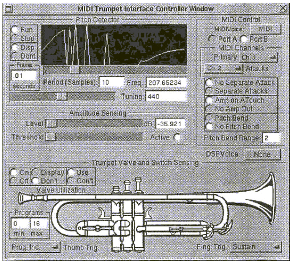
\includegraphics[width=\textwidth]{img-2-eps-converted-to-crop.pdf}
\caption{Interface panel for the Cook/Morrill Trumpet}
\label{Cook:cook-fig:1}       % Give a unique label
\end{figure}



Another project, the HIRN wind controller, sensed rotation and translation in
both hands, arm orientation, independent control with each finger, breath
pressure, and even muscle tension in the lips \cite{Cook:1992}.  Mappings from these controls
to the parameters of the WhirlWind meta-wind-instrument physical model allowed
exploration of new ``spaces'' of acoustical processes, and the HIRN also was
investigated as a controller for FM and other synthesis techniques.  Negative
lessons from the HIRN project indicated that huge control bandwidth is not
necessarily a good thing, and that attempting to build a ``super instrument''
\textit{with no specific musical composition to directly drive the project}
(\textit{principle 5}) yields interesting research questions, but with no real
product or future direction.   One positive lesson from the project is that the
\textit{co-design of synthesis/ processing algorithms with controllers} can
benefit both.

\begin{figure}[t]
\centering
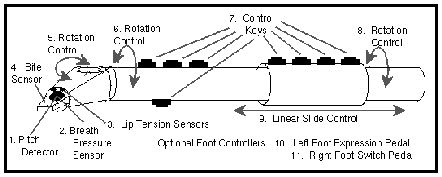
\includegraphics[width=\textwidth]{img-1-eps-converted-to-crop.pdf}
\caption{The HIRN Meta-Wind Controller}
\label{Cook:cook-fig:2}       % Give a unique label
\end{figure}


\section{Voice:  SPASM  1988--94   }

Research on physical modeling of the voice resulted in the construction of the
SPASM/Singer voice synthesizer  \cite{Cook:1991,Cook:1992a} (see Figures~\ref{Cook:cook-fig:3} and \ref{Cook:cook-fig:4}).  The SPASM system
was capable of real time synthesis, but had well over 40 continuously controlled
parameters.  Work to improve the graphical interfaces and add control via MIDI
fader boxes \cite{Cook:1993a} proved that the voice is a truly difficult ``instrument'' to
control (\textit{principles 3 \& 4}).  Recent work in real-time vocal model
control will be discussed in the SqueezeVox Section.


\begin{figure}[t]
\centering
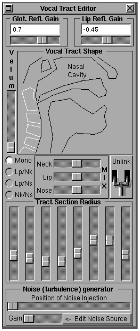
\includegraphics[height=80mm]{img-3-eps-converted-to-crop.pdf}           
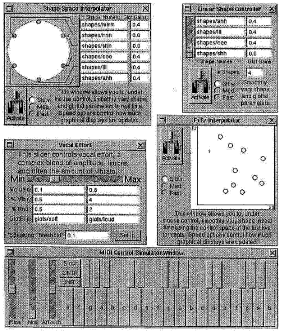
\includegraphics[height=80mm]{img-4-eps-converted-to-crop.pdf}
\caption{SPASM (left), Few-to-Many Mappings (right)}
\label{Cook:cook-fig:3}       % Give a unique label
\end{figure}



\section{PhISEM Shaker Percussion: 1996--1999}

The PhISEM (Physically Inspired Stochastic Event Modeling) project \cite{Cook:1996,Cook:1997} provided support for the ``\textit{new algorithms lead to new controllers lead to new algorithms \ldots{}}'' principles.  This work on the synthesis of particle-type percussion and real-world sounds led to a set of new instruments, not only for control of shaker/scraper sounds and sound effects, but also for algorithmic interactive music.  For example, the Frog Maraca (Figure~\ref{Cook:cook-fig:4}) sends MIDI commands to control a simple algorithmic fusion jazz combo of bass, piano, and drums.  The success with both adults and children of the Frog Maraca at Agora98 European children’s television workshop, Cyprus, Greece, came from its simple interface (just shake it), the fun of making fairly complicated music with such a simple and whimsical looking device, and the fact that it only performed one function (and always performed that function when turned on).  A related shaker percussion instrument controller was a Tambourine that could also compose algorithmic modal marimba solos when shaken.

\begin{figure}[t]
\centering
%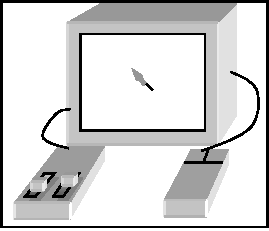
\includegraphics[width=78mm]{img-5-eps-converted-to-crop.pdf}
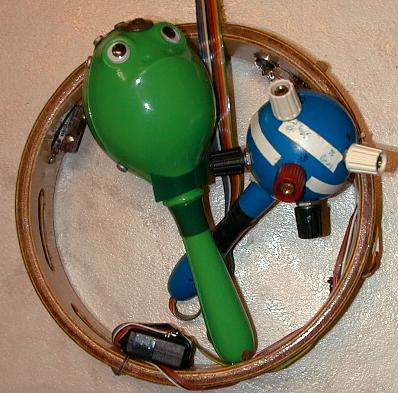
\includegraphics[width=78mm]{Figure5PhiSEM.jpg}
\caption{PhISEM controllers}
\label{Cook:cook-fig:4}       % Give a unique label
\end{figure}


Constructing the PhISEM controllers provided rich evidence that ``\textit{Programmability is a curse},'' and a correlary: ``\textit{Smart instruments are often not smart}.''  What these principles are meant to address is that the programmability of computer-based musical systems often make them too easy to configure, redefine, remap, etc.  For programmers and composers, this provides an infinite landscape for experimentation, creativity, writing papers, wasting time, and never actually completing any art projects or compositions. For normal humans, being able to pick up an instrument with a simple obvious interaction and ``play it'' only makes logical sense.  That the instrument is ``learning from their play and modifying its behavior'' often does not make any sense at all, and can be frustrating, paralyzing, or offensive.  PhISEM controllers have a single embedded microcontroller, programmed for one or two functions (selectable by the state of a button on power-up), and they put out standard General \textit{MIDI} signals.  Except for the need to replace batteries (\textit{Die Batteries Die!!}), these controllers have a strong possibility of working perfectly as designed in 10 (perhaps 20) years.  Those who craft complex systems using custom hardware, multiple computers, and multiple operating systems, can make no such claims.

\section{Foot, Hand, Kitchen Wear/Ware  1997--2000}

Spurred by the success of the PhISEM controllers, the notion of simple, MIDI
based, fixed single function controllers was continued, but based on objects that
are not specifically associated with music.  Figure~\ref{Cook:cook-fig:6} shows the TapShoe,
constructed at Interval Research as part of Bob Adams' Expressions Project.  This
shoe used force sensing resistors and accelerometers attached directly to a DSP
board running PhISEM shaker algorithms and a small rhythmic loop.  The algorithm
generated a basic ``groove'' to which the wearer of the shoe could add accents
and dynamics, in addition to their own tapping sounds.  The success of the system
came from giving the TapShoe wearer that feeling that they were actually
performing the music, though the algorithmic loop would play a relatively boring
tapping sound even if the shoe sat unworn (``\textit{Instant music, subtlety
later}'').

The Pico Glove (see Figure~\ref{Cook:cook-fig:5}) was \textit{designed as a single composition},
called ``Pico I for Seashells and Interactive Glove'' \cite{Cook:1997a}.  The idiomatic
gesture of moving the hand in and out of the shells was enhanced by a tilt sensor
in the glove.  This was used to steer fractal note-generation algorithms in real
time, to accompany the blown shells.

\begin{figure}[t]
\centering
%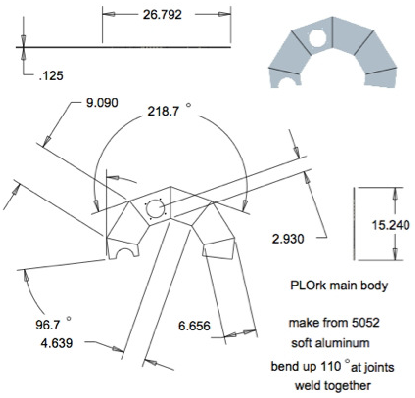
\includegraphics[width=48mm]{img-6-eps-converted-to-crop.pdf}   
%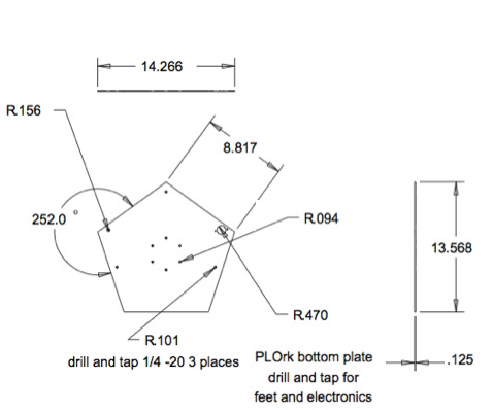
\includegraphics[width=48mm]{img-7-eps-converted-to-crop.pdf}
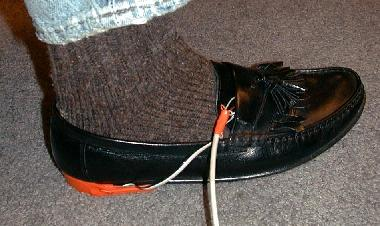
\includegraphics[height=35mm]{Figure6TapShoe.jpg}   
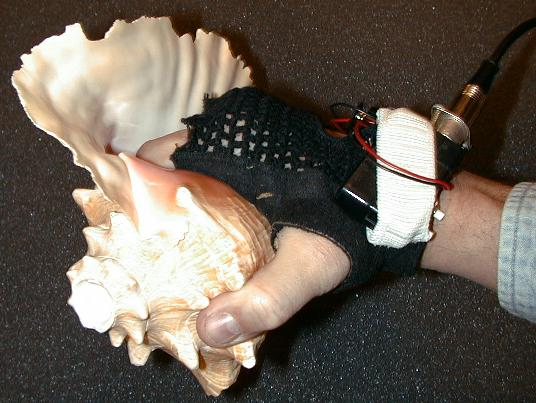
\includegraphics[height=35mm]{Figure7PicoGlov2.jpg}
\caption{Digital Tapshoe (left), PicoGlove (right)}
\label{Cook:cook-fig:5}       % Give a unique label
\end{figure}



The JavaMug (Figure~\ref{Cook:cook-fig:6}) was designed for a transcontinental MIDI jam session held
in 1997 between Tokyo and Columbia University \cite{Goto:1997}.  Being one of the author's
favorite objects, the coffee mug fits comfortably into the hand, and pressure
sensors beneath the fingers, a tilt sensor, a pot and two buttons allow control
of an algorithmic techno-latin band.   The principle of ``\textit{Instant music,
subtlety later}'' is dominant in this instrument.  Simply picking up the JavaMug
and squeezing it yields attractive and (fairly) deterministic music, because
algorithmic randomness is increased by \textit{decreasing} pressure on the
sensors.  After playing the instrument for a while, neophytes grow to more expert
levels by realizing that the music gets more varied and interesting if they
experiment with the relative pressures and tilts.  Note that this is also an
example of the ``\textit{Smart instruments are often not smart}'' principle, in
that the instrument doesn't change at all, but rather trains the user to use more
gentle and subtle manipulations of the sensors.  Other kitchen-related interfaces
include the ``Fillup Glass,'' which plays minimalist music loops (\textit{via
MIDI}) controlled by sensors in a water glass, and ``P-Ray's Caf\'{e}: Table 1''
which allows the control of a melodic percussion group by movement of common
table-top items (sugar, salt shaker, etc) over the surface of a small table. 
These objects showed that ``\textit{Everyday objects suggest amusing
controllers.}''

\begin{figure}[t]
\centering
%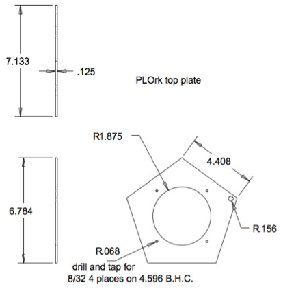
\includegraphics[width=78mm]{img-8-eps-converted-to-crop.pdf}
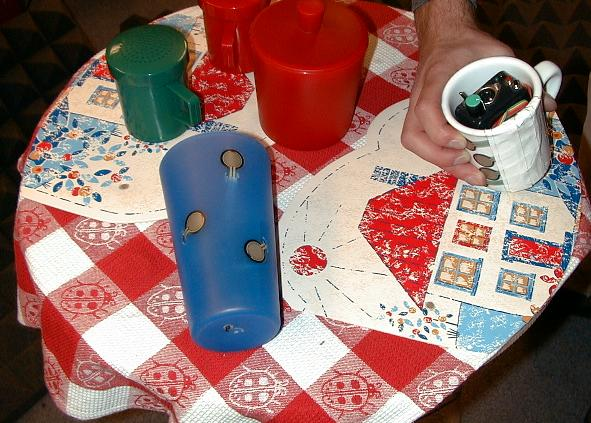
\includegraphics[width=\textwidth]{Figure8P-RaysCafe.jpg}
\caption{P-Ray's Caf\'{e}, with Fillup Glass and Java Mug}
\label{Cook:cook-fig:6}       % Give a unique label
\end{figure}


\section{Violins/Strings:  BoSSA, the Nukelele    1998--99}

Stringed instruments have a rich historical musical tradition.  They also have a
rich tradition of electronic interfaces, both commercially and experimentally
with many electrified, MIDI, and pure digital violins and guitars.  Work with Dan
Trueman at Princeton University began with a sensor-enhanced violin bow called
the ``RBow,'' and the NBody project which worked to study and model the
directional radiation properties of stringed instruments \cite{Cook:1999}.  Dan continued and
expanded this work, yielding BoSSA (The Bowed Sensor, Speaker Array, Figure~\ref{Cook:cook-fig:7})
 \cite{Trueman:1999}.  Lessons learned and reinforced by the BoSSA project include
``\textit{Existing instruments suggest new controllers},'' and ``\textit{Copying
an instrument is dumb, leveraging expert technique is smart}.'' Other principles
reinforced are ``\textit{Some players have spare bandwidth, some do not},''
(violin players generally have their hands completely occupied, so a successful
interface must exploit interesting remappings of existing gestures),  and
``\textit{Wires are not that bad (compared to wireless)}'' (the BoSSA is played
sitting by a player who often plays electric violin, so the increased complexity
of wireless was not justified).

The Nukelele (thanks to Michael Brooke for the name) was constructed in Bob
Adams' Interval Research Expressions project.  While collaborating on other
Expressions projects such as ``the Stick'' and the `` Porkophone,'' the Nukelele
was a personal experiment to design, implement, and test a new controller as
rapidly as possible.  The Nukelele was intended to match the expressiveness of a
true stringed instrument, by using audio directly from a sensor to drive a
plucked string physical model.  Two sandwiched linear force sensing resistors
under the right hand served to provide pluck/strike position information, along
with the audio excitation for the string model.

\begin{figure}[t]
\centering
%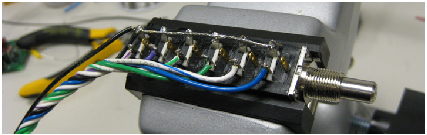
\includegraphics[width=48mm]{img-9-eps-converted-to-crop.pdf}  
%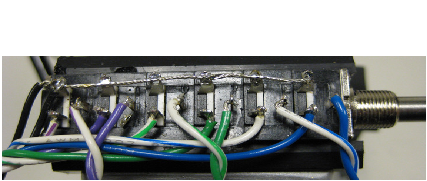
\includegraphics[width=48mm]{img-10-eps-converted-to-crop.pdf}
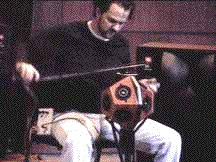
\includegraphics[height=35mm]{Figure9BoSSA.jpg}  
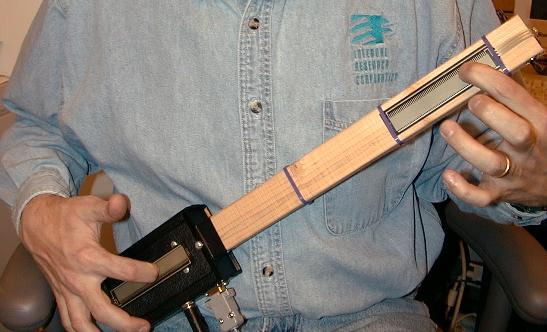
\includegraphics[height=35mm]{Figure10Nukelele.jpg}
\caption{BoSSA (left), the Nukelele (right)}
\label{Cook:cook-fig:7}       % Give a unique label
\end{figure}


\section{The Voice (again): SqueezeVox    2000}

The SqueezeVox project \cite{Cook:2000} a suitable controller for models of the human voice. 
Breathing, pitch, and articulation of vowels and consonants must be controlled in
a vocal model, so  the accordion was selected as a natural interface
(\textit{principle 10}).  Pitch via the keyboard, vibrato aftertouch, and a
linear strip for fine pitch and vibrato are controlled with the right hand. 
Breathing is controlled by the bellows, and the left hand controls vowels and
consonants via buttons (presets), or continuous controllers such as a touch pad,
plungers, or squeeze interface.

\begin{figure}[t]
\centering
%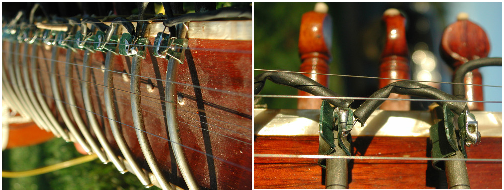
\includegraphics[width=48mm]{img-11-eps-converted-to-crop.pdf}      
%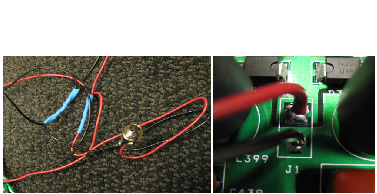
\includegraphics[width=48mm]{img-12-eps-converted-to-crop.pdf}
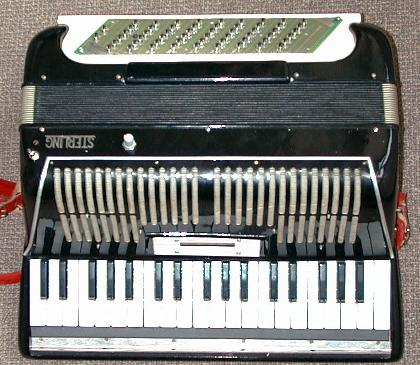
\includegraphics[height=40mm]{Figure11SQBart.jpg}      
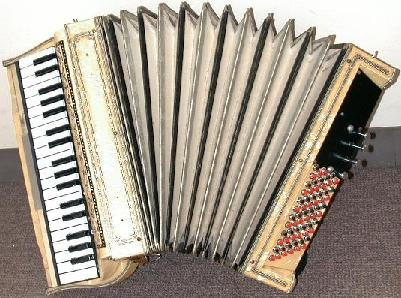
\includegraphics[height=40mm]{Figure11SQLisa.jpg}
\caption{Squeezevox Lisa (left) and Bart (right)}
\label{Cook:cook-fig:8}       % Give a unique label
\end{figure}



\section{Future Work  and Conclusions}

Work and development continues on the SqueezeVox project, with a self-contained
version (Santa's Little Helper, with onboard DSP synthesis), and a small
concertina version (Maggie) currently under construction.  Work also continues on
the kitchen/common objects project, and given the variety of such objects, much
rich interface and music design lies ahead.

Musical interface construction proceeds as more art than science, and possibly
this is the only way that it can be done.  Yet many of the design principles put
forth in this paper have held true in multiple projects, and many have been
verified in talking with other digital instrument designers.  Some of the
technological issues might go away, but not completely or not necessarily very
quickly.  Many of the human/artistic issues are likely to be with us as long as
musical instruments have been.

\section{Demonstrations}

During the workshop, the PhISEM controllers, the JavaMug, the TapShoe, the
Nukelele, and the SqueezeVox will be demonstrated.  Soundfiles, large pictures,
% Origintal text:
%and video clips of the instruments discussed in this paper are available at: 
%\href{http://www.cs.princeton.edu/~prc/CHI01.html}{http://www.cs.princeton.edu/~prc/CHI01.html}
% edited to: 
and video clips of the instruments discussed in this paper are available online.\footnote{\url{http://www.cs.princeton.edu/~prc/CHI01.html}}

\begin{acknowledgement}
Specific thanks to Dexter Morrill, Dan Trueman, Bob Adams, and Colby Leider. 
General thanks to all those at CCRMA, Princeton, and Interval Research for
wonderful collaborations.  This work was funded by CCRMA and the CCRMA Industrial
Affiliates Program, Interval Research, Intel, and the Arial Foundation.
\end{acknowledgement}



\section*{Author Commentary: NIME: 15 years later. Wow!}

\paragraph{Perry Cook}


What a run it's been.  I could never have imagined that this paper might become one of my most cited and downloaded publications, but I guess it makes sense for a variety of reasons.  Here I ponder some of those reasons, and give some thoughts on the time since.

First, it was the very first NIME, actually the ACM/CHI workshop, before the NIME organization and conference itself began running autonomous from ACM CHI.  So the network effect of being one of the first papers helps a lot.

I won't pretend that the information in this paper was particularly sage or epic by any means, but it did provide a good introductory reader and reference for a new curriculum area just getting started in music tech programs around the world.  Long before NIME (5 or 10 years or more before) there were courses like Dan O'Sullivan's Physical Computing course at ITP/NYU, and some other HCI Technology courses (like the multi-university San Jose State + CCRMA + Princeton + others course that Ben Knapp and Dick Duda \cite{Knapp:1995} got started with many of us back in 1996).  But with the birth of NIME, courses like this could be re-focussed on music (the true goal for many of us all along), so having a NIME course made sense for many music technology and digital arts curricula.

This paper came before a lot of other cool things that happened in my academic and artistic life.  Most of the experiences that brought about my 2001 list of NIME Principles came from working with NIME builders: at CCRMA, and with DanO, Bob Adams, Michael Brook, Geoff Smith, Dan Levitin, Bill Verplank, and others at Interval Research \cite{Levitin:2002}, and Ben Knapp and others on our own HCI Technology courses \cite{Knapp:1995}.  Princeton and my DSP+NIME curriculum brought me Dan Trueman and BoSSA, Ge Wang and ChucK, many (hemi)spherical speakers with Dan, Scott Smallwood, Curtis Bahn, Stephan Moore and others, the Princeton Laptop Orchestra (and many other LORks), Ajay Kapur and his Karmetik Robots and Machine Orchestra, Rebecca and Wekinator, many other great students, and lots of other NIME developments.

Finally, I updated the paper subsequently with new insights, revisions, and corrections based on changing technology or a different vantage point on my part.

My NIME 2007 Keynote at NYU, titled: ``Principles for Controlling Computer Music Designers,'' \cite{Cook:2007} took a look at teaching a NIME curriculum, and early lessons from the Princeton Laptop Orchestra.  So I added some new principles:  

\begin{enumerate}
 \setcounter{enumi}{14}
	\item More can be better (but hard) (PLORk went from an initial 15 members,  to 35!)
	\item Music+Science is a great teaching/marketing tool (important in academic jobs)
	\item The younger the student, the more fearless (they don't know/care what's hard)
\end{enumerate}

My NIME 2009 paper, ``Re-Designing Principles for Computer Music Controllers: a Case Study of SqueezeVox Maggie,'' \cite{Cook:2009} was about revisiting some older versions of my NIME instruments and my experiences with actually re-designing/re-building them.  And of course, I changed one: 

\begin{enumerate}
 \setcounter{enumi}{12}
	\item (b) Funny is often much better than serious (whimsical designs are not a crime)
\end{enumerate}

\noindent
and added even more new principles:

\begin{enumerate}
 \setcounter{enumi}{17}
\item Redesign for backward compatibility (make sure you can play your old pieces)
\item Design (and pack) for post-9/11 travel (document, make sure things demo easily)
\item (a) Build a (new) copy, don't trash the original (keep it around to compare), and (b) Build two or more if you can afford it. (one will invariably work better)
\item Wire and document for future surgeries  (labeled 20 in paper, should be 21)
\item Build in diagnostic features and displays (labeled 21, should be 22)  
\item Construct controller proxies (functional GUIs) (labeled 22, should be 23)
\end{enumerate}

So one additional (personal) principle that I would add has to do with double-checking the numbering of lists in papers and sequels.  Another principle might be that we never know where a piece of work, or publication, or small workshop as an adjunct to a larger conference, might lead.  The ACM/CHI New Interfaces for Musical Expression workshop turned into something bigger than any of us might have dreamed.

I'm really happy to have been a part of the NIME history (so far).  All indications are that we've still got a lot ahead of us.


\section*{Expert Commentary: Perry Cook's Principles Still Going Strong}

%\paragraph{Marcelo M. Wanderley, McGill University, marcelo.wanderley@mcgill.ca}
\paragraph{Marcelo M. Wanderley}

The NIME 2001 workshop was a very interesting venue. A rather active musical controllers community already existed for several years in 2001—mostly active at the International Computer Music Conference (ICMC), with key papers in the area already published before the NIME workshop (including many by Perry himself. See the electronic book ``Trends in Gestural Control of Music'' for a state of the art in 2000).\footnote{\url{http://www.idmil.org/projects/trends}} Even so, the NIME 2001 workshop was a unique opportunity to meet researchers directly working in this area, see demos of their work at the Experience Music Project in Seattle, and discuss possible ways to organize a research community around it. Several of the papers presented in the workshop became main references in our field, with several hundred citations each: Perry's, Wessel and Wright's \cite{Wessel:2001} and Orio et al.'s \cite{Orio:2001}, the two last ones with sequels published in the 2002 Computer Music Journal special edition (vol. 26, number 3) on NIME.

It was very interesting to re-read Perry Cook's 2001 NIME workshop paper, as well as its NIME 2009 follow up paper where he reviews the original 2001 guidelines in light of newer developments. Perry's 2001 paper belongs to a tradition of works from builders/performers (or performer/builders) who excel in both areas. Such works have the advantage of bringing to the community lots of personal, first hand performance experience informed by a strong technical/scientific component. In this sense, it is complementary to works by designers who mostly focus on technical aspects, who nevertheless collaborate with (multiple) artists when designing their devices. The advantage of the later group is that one can (hopefully!) more easily avoid one's own aesthetic ideas about music and art and provide a larger, albeit forcefully less coherent, set of examples from which to derive guidelines. The study of both approaches, taking into consideration their own strengths and limitations, should lead to interesting (and informed!) designs. 


It is amazing to see that in almost 15 years, many (most?) of its principles and guidelines still hold true. My favorites are (\#4) ``Some players have spare bandwidth, some do not'' (true, how true!), (\#2) ``Smart instruments are often not smart,'' (\#1) ``Programmability is a curse,'' and (\#6) ``Instant music, subtlety later.'' The last one ties well to Wessel and Wright's principle: ``Low entry fee, with no ceiling on virtuosity'' \cite{Wessel:2001}.


Being part of the group who focuses mostly on technical issues (an example of a great paper about design is \cite{Bongers:2000}), I am less in agreement with principle \#5 (``Make a piece, not an instrument or controller''), as I have seen many interesting instruments made without a musical piece in mind, but that subsequently were extensively used musically. The case in mind is Joe Malloch's t-Stick \cite{Malloch:2007}, who in collaboration with composer/performer D. Andrew Stewart, developed a device that became an established instrument used in dozens of musical pieces (check Andrew's impressive t-stick performance videos at vimeo.com). 

I also take principles \#10 and \#11 (``New algorithms suggest new controllers'' and ``New controllers suggest new algorithms'') with a grain of salt, as I believe that they underplay the idea importance of mapping (between controller outputs and algorithm inputs). Complex mapping strategies can provide tools to use a variety of algorithms with the same controller (e.g. \cite{Hunt:2002}), leading to interesting instruments. Furthermore, not all instrument designers are proficient in sound design and might just want to use algorithms they are familiar with, even when using different controllers (and conversely).

Finally, other principles seem to have become less useful with time, as for instance, battery life that has dramatically improved in the last 15 years (\#8), making the use of cables is less necessary in instrument design (although still useful in many occasions!) (\#9). In short, this is still a very useful, inspiring paper. Perry's direct style is excellent and the review of his previous works until then is enlightening. Some of its principles will hold for a long time (forever?) and have become basic bricks to our community. 

